\chapter{Propuesta}\label{chapter:proposal}

En este capítulo, se aborda la implementación práctica del modelo \textbf{TrajBERT}, explorando sus fortalezas y limitaciones en el completamiento de trayectorias humanas. Para ello, se detalla el proceso de diseño e implementación del modelo, desde el preprocesamiento de los datos hasta la configuración de su arquitectura. Adicionalmente, se evalúan las capacidades técnicas de \textbf{TrajBERT} mediante su aplicación a la base de datos pública HuMob Challenge 2023, lo que permite obtener una línea base de desempeño antes de su adaptación a las particularidades del contexto cubano.

El desarrollo de este capítulo se estructura de la siguiente manera: primero, se incluye una definición formal del problema a resolver y se describe la arquitectura y los fundamentos del modelo \textbf{TrajBERT}, destacando sus componentes clave y las razones de su elección para este estudio. A continuación, se presenta el preprocesamiento de los datos y las métricas de evaluación utilizadas para medir el desempeño del modelo. Finalmente, se analizan los resultados obtenidos en esta etapa inicial de implementación, estableciendo una base para las adaptaciones posteriores en el contexto local que serán abordadas en el siguiente capítulo.

\section{TrajBert}

El modelo TrajBert fue desarrollado por Si et al. en \cite{si2023trajbert} en enero del 2023, para abordar el problema de completamiento de trayectorias humanas. Este modelo destaca por su capacidad para aprender patrones de movilidad de manera bidireccional, refinando las predicciones a través de un proceso de combinación con puntos vecinos conocidos en la trayectoria e incorporando una novedosa función de pérdida consciente del espacio y el tiempo. En los experimentos realizados sobre conjuntos de datos del mundo real, TrajBERT demostró una mejora de al menos un 8.2\% en comparación con los métodos más avanzados de recuperación de trayectorias disponibles hasta la fecha y en trayectorias extremadamente escasas, como el caso del contexto cubano, resalta su potencial como una herramienta práctica y efectiva en el análisis de la movilidad humana.

\subsection{Preliminares}

Las trayectorias sin procesar son dispersas, no uniformes y presentan variabilidad en el tamaño de la secuencia. Por tanto, en \cite{si2023trajbert} se consideró fundamental partir de una definición formal del problema a resolver. Las definiciones relacionadas se presentan a continuación.

\begin{definition}{ID de Ubicación:}
    Un ID de ubicación corresponde a una región geográfica pero carece de información geográfica explícita, como coordenadas. Puede ser un ID de celda de una estación base, un ID único de Wi-Fi o un identificador único universal (UUID) generado por un generador de números aleatorios.
\end{definition}

\begin{definition}{Trayectoria Implícita:}
    Una trayectoria implícita $T$ se define como una secuencia ordenada temporalmente de IDs de ubicación generada dentro de un día, representada como $T = \{p_1, p_2, \ldots, p_j, \ldots, p_n\}$, donde $p_j$ es el $j$-ésimo punto de la trayectoria, representado como $p_j = (\loc_j, \text{ts}_j)$, siendo $\loc_j$ el ID de ubicación, $\text{ts}_j$ la marca temporal cuando se registró el punto de la trayectoria, y $n$ el número total de puntos registrados.
\end{definition}

\begin{definition}{Trayectoria Muestreada con Intervalo $\epsilon$:}
    Una trayectoria muestreada con intervalo $\epsilon$ se representa como $T_\epsilon = \{\loc_1, \loc_2, \ldots, \loc_j, \ldots, \loc_m\}$, donde $m$ es el número total de intervalos de muestreo en un día. $\epsilon$ es el intervalo de muestreo, es decir, la diferencia de tiempo entre IDs de ubicación consecutivos. La definición del valor de $\epsilon$, así como el tamaño de la ventana de tiempo que se analizará, definirá la cantidad máxima de IDs de ubicación efectivas en una trayectoria. Si falta el ID de ubicación en un intervalo de muestreo $j$, $\loc_j$ será reemplazado por un signo predefinido \emph{PAD}.
    \label{def:e_sampling}
\end{definition}

% \subsection*{Planteamiento del Problema}

Finalmente, dada una trayectoria implícita $T$ no uniforme, el \textbf{objetivo} del modelo es recuperarla para obtener una trayectoria muestreada con intervalo $\epsilon$, $T_\epsilon$, prediciendo los IDs de ubicación de los intervalos de muestreo faltantes de manera que se asemeje lo más posible a la ruta de movimiento real del usuario.

\subsection{Arquitectura}

Inspirados por el éxito del modelo BERT \cite{devlin2018bert} en el procesamiento de lenguaje natural, el modelo TrajBERT utiliza el \textit{encoder} de \cite{vaswani2017attention} como red base y el enfoque de \textit{Masked Language Model} (MLM) para su entrenamiento. La idea principal es que si BERT es capaz de completar palabras faltantes en una oración, una arquitectura similar que aproveche los datos espaciotemporales, podrá completar satisfactoriamente puntos faltantes en una trayectoria. Su arquitectura, reflejada en la figura \ref{fig:trajbert_architecture}, consta de tres componentes principales: una capa de preprocesamiento que transforma las trayectorias implícitas, escasas y no uniformes en trayectorias uniformes con muestreo $\epsilon$; un codificador de trayectorias que aprende las representaciones ocultas de las ubicaciones faltantes utilizando el codificador Transformer y un esquema de refinamiento temporal local; y una capa de salida diseñada para predecir las ubicaciones faltantes, incorporando dependencias espaciales y temporales mediante una función de pérdida. Estos módulos trabajan de manera conjunta para abordar el problema de recuperación de trayectorias humanas con alta precisión.

\begin{figure}[!htb] \centering 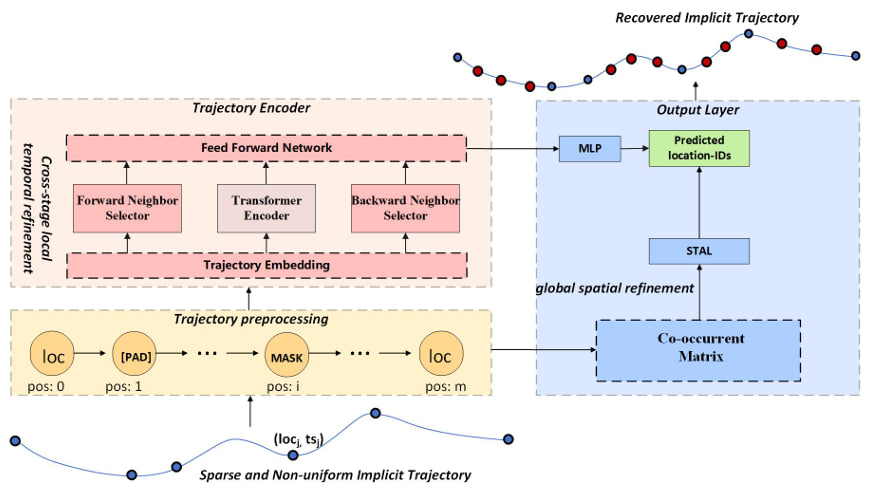
\includegraphics[width=1\textwidth]{Graphics/trajbert_architecture.jpg} \caption{Arquitectura de TrajBert, figura extraída de \cite{si2023trajbert}.} \label{fig:trajbert_architecture} 
\end{figure}

\subsubsection{Preprocesador de trayectorias}

El problema de recuperación de trayectorias enfrenta importantes desafíos debido a la naturaleza no uniforme y de longitud variable de las trayectorias, que presentan patrones de movilidad con granularidades diversas y brechas temporales entre registros consecutivos que pueden variar desde segundos hasta horas. Para abordar esta problemática, en \cite{si2023trajbert} proponen transformar las trayectorias implícitas originales en trayectorias con muestreo $\epsilon$, permitiendo trabajar con entradas de longitud fija. En este enfoque, cada trayectoria se segmenta en intervalos temporales basados en la marca de tiempo (\textit{timestamp}) de cada punto, como se detalla en la ecuación ~\ref{eq:segments}:

\begin{equation}
\text{seg}_i = \cup \{ \loc_j \mid \text{ts}_j \% 86400 / \epsilon = i \}
\label{eq:segments}
\end{equation}

Donde $i$ representa el $i$-ésimo intervalo de tiempo, $\text{seg}_i$ corresponde al segmento de trayectoria dentro de ese intervalo, y $\epsilon$ define la duración de cada intervalo de tiempo. En el caso de intervalos con múltiples valores de \textit{ID de ubicación}, los autores seleccionan el valor más frecuente como representante. Para los intervalos sin registros, se introduce un signo predefinido (\textit{‘PAD’}). Finalmente, estas trayectorias con muestreo $\epsilon$ se representan como $T_\epsilon = \{\loc_1, \loc_2, \cdots, \loc_j, \cdots, \loc_m\}$, sirviendo como entradas para la capa de codificación de trayectorias.

\subsubsection{Codificador de trayectorias}

Según lo descrito por los autores en \cite{si2023trajbert}, la recuperación de trayectorias comparte similitudes con el \textit{cloze task}\footnote{El \textit{cloze task} es un método de evaluación que mide la habilidad de los participantes para completar un texto que contiene palabras omisas, asegurando la comprensión contextual de la información presentada.} en el procesamiento de lenguaje natural. Ambas requieren predecir elementos faltantes (tokens o \textit{ID de ubicación}) utilizando información anterior y posterior en la secuencia. En este caso, el objetivo es definir una función de mapeo $f$ para predecir el \textit{ID de ubicación} del $i$-ésimo intervalo de tiempo, con base en las trayectorias con muestreo $\epsilon$ como entrada, de forma que ${pred\_loc}_i = f(i, T_\epsilon)$.

Para lograrlo, se emplea el \textit{encoder} de Transformer junto con un esquema de refinamiento temporal local. Este codificador bidireccional utiliza un mecanismo de atención multi-cabeza, lo que permite considerar puntos de la trayectoria en ambas direcciones y modelar de manera efectiva patrones de movilidad espacio-temporales. Durante el entrenamiento, los autores aplican la técnica de enmascaramiento propuesta en BERT, donde un 15\% de los \textit{ID de ubicación} efectivos se enmascaran aleatoriamente, omitiendo los intervalos marcados como ‘PAD’. Los \textit{ID de ubicación} enmascarados se configuran como ‘MASK’ con un 80\% de probabilidad, se mantienen iguak en un 10\% y como un \textit{ID de ubicación} aleatorio en el 10\% restante.

Para alimentar las trayectorias al \textit{encoder}, se convierten los \textit{ID de ubicación} y los índices de los intervalos de tiempo en representaciones densas mediante una capa de \textit{embeddings} entrenable. Estos \textit{embeddings} se combinan con codificaciones posicionales para formar los vectores de entrada:

\begin{equation}
E_{T_\epsilon} = E_{\loc} + E_{\text{pos}}
\end{equation}

El \textit{encoder} utiliza múltiples capas con mecanismos de atención para aprender patrones espaciotemporales bidireccionales y cada capa aplica normalización, redes de avance y activaciones \textit{Gelu} para generar representaciones ocultas de las trayectorias.

Para mejorar la precisión en la recuperación de trayectorias, los autores diseñan un esquema de refinamiento espaciotemporal que enfatiza los \textit{ID de ubicación} vecinos recientemente visitados y próximos por visitar. Este enfoque incorpora vectores de \textit{embedding} de los vecinos más cercanos hacia adelante y hacia atrás de los puntos faltantes, pero como un resultado independiente del \textit{encoder}, para evitar sesgos. Finalmente, estos \textit{embeddings} se combinan con las representaciones vectoriales ocultas aprendidas por el \textit{encoder}. Esta idea resulta ser el primer aporte de \cite{si2023trajbert} al campo del completamiento de trayectorias, y se basa en que los puntos que más influyen en una trayectoria sobre un token faltante, son justamente sus vecinos inmediatos en ambas direcciones.

% destacando cómo la incorporación de dependencias locales mejora significativamente la precisión en la predicción de puntos faltantes. Al combinar patrones espacio-temporales globales aprendidos por el \textit{encoder} con información detallada de vecinos inmediatos, el enfoque aborda las limitaciones de modelos previos que ignoraban el impacto del contexto local en los datos secuenciales.

\subsubsection{Capa de salida}

La capa de salida de TrajBERT introduce una novedosa función de pérdida para incorporar dependencias espaciales globales en el entrenamiento del modelo. 

\begin{figure}[!htb] \centering 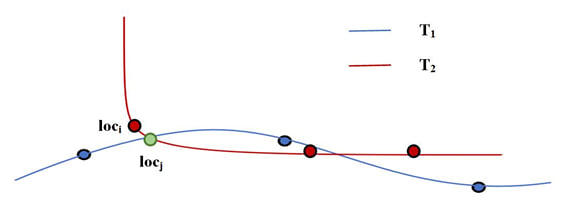
\includegraphics[width=0.5\textwidth]{Graphics/co_ocurrent_trajectories.jpg} \caption{$loc_i$ y $loc_j$ co-ocurren frecuentemente, son espacial y temporalmente contiguos, figura extraída de \cite{si2023trajbert}} \label{fig:co_ocurrent_trajectories} 
\end{figure}

Si dos \textit{ID de ubicación} (\(\loc_i\) y \(\loc_j\)) co-ocurren frecuentemente en trayectorias, se consideran contiguos tanto espacial como temporalmente, representando áreas geográficamente cercanas. Por ejemplo, en \ref{fig:co_ocurrent_trajectories} el punto $loc_j$ de $T_1$ co-ocurre frecuentemente con $loc_i$ en otras trayectorias, ambos puntos son cercanos geográficamente. A partir de esta relación de co-ocurrencia, se construye una matriz \(H\), definida como:

\begin{equation}
H[\loc_i][\loc_j] = \frac{co_{\loc_i, \loc_j}}{\sum_{l} co_{\loc_i, l}},
\label{eq:co_ocurrence_matrix}
\end{equation}

\noindent
donde \(co_{\loc_i, \loc_j}\) es el valor de co-ocurrencia entre \(\loc_i\) y \(\loc_j\).

La salida del modelo asigna a cada \textit{ID de ubicación} posible una probabilidad, la cual es inicialmente optimizada mediante una función de pérdida estándar basada en entropía cruzada (\textit{Cross Entropy Loss}, \(CEL\). Sin embargo, esta función no diferencia entre predicciones geográficamente cercanas y lejanas al valor real, lo que puede resultar en penalizaciones injustas para predicciones que representan ubicaciones cercanas al objetivo real.

Para abordar este problema, \cite{si2023trajbert} propone una función de pérdida consciente del espacio y tiempo (\textit{Spatial-Temporal Aware Loss}, \(\text{STAL}\)), que incorpora las estructuras espaciales globales aprendidas de la matriz \(H\). \(\text{STAL}\) está definida como:

\begin{equation}
\text{STAL} = \beta_1 \cdot L_1 + \beta_2 \cdot L_2,
\label{eq:stal}
\end{equation}

\noindent
donde \(L_1\) ajusta las penalizaciones para predicciones cercanas geográficamente utilizando un coeficiente espacio-temporal \(w(loc_i, loc_j)\), calculado como:

\begin{equation}
    L_1 = - \sum_{i=1}^N \sum_{j=1}^M \sum_{k=1}^S \sigma_{i,j,k} \log \left( P(\loc_{i,j,k} \mid T^\epsilon_i, \theta) \right),
\end{equation}

\begin{equation}
    \sigma_{i,j,k} = \left( 1 - P(t_{i,j} \mid T^\epsilon_i, \theta) \right) \cdot \left( 1 - w(t_{i,j}, \loc_{i,j,k}) \right),
\end{equation}

\begin{equation}
    w(\loc_i, \loc_j) =
    \begin{cases} 
        1, & \text{si } \loc_i = \loc_j, \\
        \displaystyle \frac{\exp(H[\loc_i][\loc_j] / \mu)}{\sum_s \exp(H[\loc_i][\loc_s] / \mu) + \eta}, & \text{si } H[\loc_i][\loc_j] > \gamma, \\
        0, & \text{en otro caso.}
    \end{cases}
\label{eq:w_loc_cases}
\end{equation}

\noindent
aquí, \(\gamma\) es un umbral de co-ocurrencia, \(\mu\) es un parámetro de escala y \(\eta\) es una constante. \(L_2\) corresponde a la entropía cruzada estándar. Esta función de pérdida reduce las penalizaciones para predicciones cercanas geográficamente al valor real, alineándose con las restricciones de movilidad humana impuestas por las estructuras espaciales de las ciudades.

\subsection{Implementación}

El modelo se implementó utilizando Python 3.12.4 y PyTorch (2.3.1+cu118) y se basó en un repositorio público disponible en \href{https://r.search.yahoo.com/_ylt=AwrihnbEpIxnbfEg4Q8PxQt.;_ylu=Y29sbwNiZjEEcG9zAzEEdnRpZAMEc2VjA3Ny/RV=2/RE=1737299269/RO=10/RU=https%3a%2f%2fgithub.com%2fTrajResearch%2fTrajBERT/RK=2/RS=d0fhOp0ellpCiDBR7qVYR9S3bFY-}{GitHub}, que sirvió como punto de partida para este trabajo. Sin embargo, el código original presentaba múltiples desafíos que requerían una revisión profunda y adaptaciones significativas para ajustarse a los objetivos del estudio. La falta de documentación en el repositorio dificultaba la comprensión del flujo general del modelo, por lo que fue necesario analizar minuciosamente cada componente del código para comprender su funcionalidad.

Otro desafío importante fue que la arquitectura y las métricas del modelo estaban diseñadas para un dominio de datos diferente, por lo que fue imprescindible reescribir funciones clave relacionadas con el preprocesamiento, la tokenización y el manejo de datos. Además, se eliminaron secciones del código que resultaban redundantes o innecesarias, optimizando así el tiempo de ejecución y reduciendo el consumo de memoria. Durante este proceso, se realizaron pruebas exhaustivas, tanto unitarias como con datos reales, para garantizar la robustez del sistema y corregir errores que no estaban contemplados en el diseño original. Por ejemplo, algunos ajustes implicaron la reestructuración del flujo de entrenamiento y evaluación, la incorporación de manejo eficiente de memoria en GPU y la implementación de validaciones adicionales para garantizar la coherencia en los resultados.

Finalmente, se mejoró la documentación del código, incluyendo comentarios detallados y explicaciones de los parámetros. Este paso no solo facilitó la comprensión del modelo, sino que también permitió reutilizar y expandir su funcionalidad en futuros trabajos. El proceso de implementación no fue simplemente una reproducción del código existente, sino una adaptación profunda y consciente que involucró modificaciones técnicas y mejoras en la eficiencia, lo que resultó en un modelo funcional, optimizado y alineado con los objetivos de este trabajo.

\subsection{Opinión}

El modelo \textbf{TrajBERT} presenta una arquitectura robusta y bien diseñada para el completamiento de trayectorias y reconocimiento de patrones humanos. Su enfoque basado en Transformers, combinado con el refinamiento espaciotemporal y la función STAL, suponen una solución prometedora en contextos donde la información disponible es limitada.

Sin embargo, desde el punto de vista de su diseño, \textbf{TrajBERT} presenta algunas limitaciones que mitigan el valor contextual que ofrecen otros datos relativos a las trayectorias. En primer lugar, no está diseñado para aprovechar el conocimiento sobre qué usuario realizó cada trayectoria, lo cual restringe la capacidad del modelo para personalizar las predicciones o identificar patrones específicos de usuarios individuales. En segundo lugar, la arquitectura no considera información temporal como el día de la semana, lo que podría ser crucial para detectar patrones periódicos en los datos, como trayectorias relacionadas con rutinas laborales o actividades recreativas recurrentes. Por último, el modelo no incorpora explícitamente el papel de los puntos de interés en las distintas zonas geográficas, lo que podría ser relevante para entender las motivaciones detrás de las trayectorias y capturar relaciones espaciales significativas en los datos.

Aunque estas observaciones no se basan en experimentos específicos, sino en un análisis teórico de la arquitectura, sugieren áreas de mejora que podrían potenciar aún más la eficacia del modelo en aplicaciones futuras. Incorporar estas dimensiones contextuales en el diseño de \textbf{TrajBERT} podría ampliar significativamente su capacidad para capturar dinámicas más complejas y proporcionar predicciones más precisas en escenarios reales.

\section{Aplicacion a datos del challenge Japones}

En esta sección, se describe la implementación de \textbf{TrajBERT} sobre un conjunto de datos real proveniente de la competencia Humob en su edicion del 2023. Inicialmente, se presentan las principales estadísticas de los datos, destacando los factores que influyeron en las decisiones tomadas durante el proceso de diseño y entrenamiento del modelo. Posteriormente, se analizan los resultados obtenidos en los experimentos realizados, comparando el desempeño de \textbf{TrajBERT} con enfoques tradicionales. Finalmente, se discuten las conclusiones obtenidas, resaltando las ventajas de esta arquitectura en contextos reales.

\subsection{Humob}

El \textit{Human Mobility (HuMob)}  Challenge es una competencia internacional que busca evaluar y mejorar los modelos computacionales para la predicción de patrones de movilidad humana. Utilizando conjuntos de datos abiertos y de gran escala, que reflejan trayectorias de movimiento humano en áreas metropolitanas, este desafío proporciona a los investigadores una plataforma estandarizada para desarrollar y probar sus métodos de predicción. Los participantes reciben datos de movimiento de individuos durante un período determinado, segmentados en intervalos de 30 minutos. El objetivo es predecir los movimientos de un subconjunto de individuos en ciertas ciudades durante días específicos, utilizando datos históricos de movimiento tanto de la misma ciudad como de otras.

Para facilitar el desarrollo de modelos de predicción, se proporciona información adicional sobre los puntos de interés (\textit{Points of Interest}, POI) en cada celda de la cuadrícula, representada por vectores de múltiples dimensiones. Aunque las categorías específicas de los POI no se divulgan, esta información puede ser útil para capturar patrones de movilidad relacionados con la infraestructura urbana. La evaluación de las predicciones se realiza comparando las trayectorias previstas con las reales, utilizando métricas como GEO-BLEU \cite{shimizu2022geo} y \textit{Dynamic Time Warping} (DTW) \cite{muller2007dynamic}. Estas métricas permiten medir la precisión de las predicciones desde diferentes perspectivas, considerando tanto la similitud local como la alineación temporal de las trayectorias. 

El HuMob Challenge no solo promueve la innovación en la modelización de la movilidad humana, sino que también fomenta la colaboración y el intercambio de conocimientos entre investigadores de diversas disciplinas. Al proporcionar un conjunto de datos común y un marco de evaluación estandarizado, la competencia facilita comparaciones justas entre diferentes enfoques y contribuye al avance colectivo en la comprensión y predicción de los patrones de movilidad urbana. Los datos usados en este experimento son los publicados en su edición del 2023.

\subsection{Set de datos}

El conjunto inicial de datos fue curado mediante un recorte espacial y temporal de datos brutos de telefonía móvil. Se definió un área delimitada alrededor de una ciudad en Japón, seleccionando usuarios que fueron observados dentro de esta área al menos 10 veces durante un período de 10 días. Para preservar el anonimato, las ubicaciones se discretizaron en celdas de 500 m × 500 m, los tiempos se agruparon en intervalos de 30 minutos y las fechas exactas se enmascararon. Los datos registran el movimiento de los usuarios durante 60 días de actividad normal y 15 días durante una situación de emergencia. Solo se incluyeron usuarios con un número suficiente de observaciones, resultando en 25,000 usuarios. Las observaciones fuera del área delimitada fueron descartadas. En este estudio solo se usaron los primeros 5,000 usuarios y las trayectorias de sus primeros 60 días de actividad normal. 

\begin{figure}[!htb]
\centering
\begin{minipage}{0.5\textwidth}
    \centering
    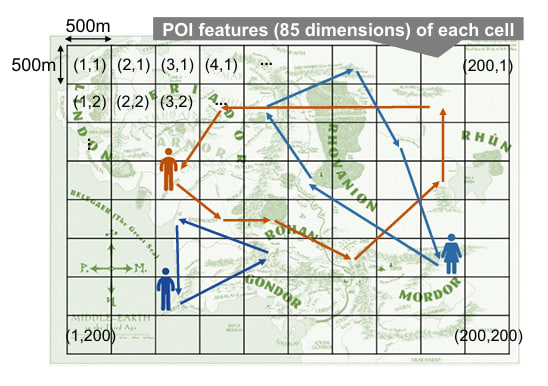
\includegraphics[width=\textwidth]{Graphics/humob_matrix_mobility.jpg}
    \caption{Las trayectorias fueron discretizadas en celdas de 500 m × 500 m en una matriz de 200 x 200 celdas, figura extraída de \cite{yabe2024yjmob100k}.}
    \label{fig:humob_matrix_mobility}
\end{minipage}%
\hfill
\begin{minipage}{0.45\textwidth}
    \centering
    \begin{tabular}{|c|c|c|c|c|}
    \hline
    \textbf{uid} & \textbf{d} & \textbf{t} & \textbf{x} & \textbf{y} \\ \hline
    1 & 10 & 31 & 7 & 10 \\ \hline
    1 & 10 & 32 & 7 & 10 \\ \hline
    1 & 10 & 33 & 8 & 9  \\ \hline
    1 & 10 & 34 & 9 & 13 \\ \hline
    1 & 10 & 35 & 8 & 8  \\ \hline
    1 & 10 & 37 & 8 & 8  \\ \hline
    1 & 10 & 38 & 7 & 8  \\ \hline
    \multicolumn{5}{|c|}{\dots} \\ \hline
    \end{tabular}
    \captionof{table}{Ejemplo de los datos del conjunto de usuarios y sus ubicaciones discretizadas.}
    \label{tab:humob_example_data}
\end{minipage}
\end{figure}

La tabla \ref{tab:humob_example_data} muestra un ejemplo del conjunto de datos proporcionado. Cada registro representa una observación de un individuo y consta de las siguientes columnas:

\begin{itemize}
    \item El ID de usuario es un identificador único para cada usuario de teléfono móvil.
    \item El día corresponde a la fecha enmascarada de la observación, que puede variar entre 0 y 59 en ambos conjuntos de datos.
    \item El intervalo de tiempo representa la marca temporal discretizada en intervalos de 30 minutos, con valores entre 0 y 47; por ejemplo, 0 indica el intervalo entre las 00:00 y 00:30 horas, mientras que 13 corresponde al intervalo entre las 6:30 y 7:00 horas.
    \item Las coordenadas x, y indican la ubicación observada mapeada en una cuadrícula discretizada de 500 metros, con valores que van de (1, 1) a (200, 200), como se ilustra en la figura \ref{fig:humob_matrix_mobility}.
\end{itemize}

El número total de registros es 4,999,742 entre los 5,000 usuarios. La figura \ref{fig:unique_cell_per_user_histogram} muestra un histograma del número de celdas únicas visitadas por usuarios, se visualiza una distribución sesgada, donde una pequeña fracción de los usuarios es observada muchas veces. La figura \ref{fig:unique_user_per_cell_histogram} muestra el histograma del número de usuarios únicos que visitaron cada celda, el eje x está en escala logarítmica. El gráfico muestra que una fracción de las celdas son visitadas muy pocas veces (menos de 10 usuarios únicos), mientras que se puede observar otra acumulación alrededor de los 100 usuarios únicos, lo cual resalta la mezcla de áreas urbanas y rurales en la región estudiada.

\begin{figure}[!htb]
\centering
\begin{minipage}{0.45\textwidth}
    \centering
    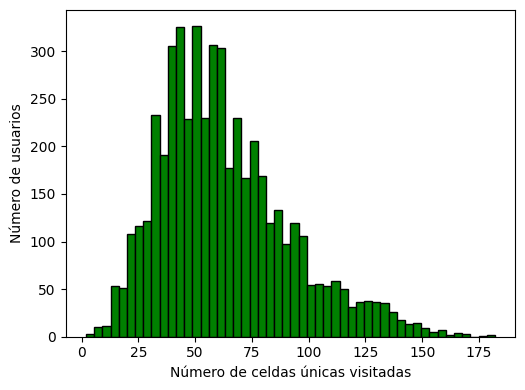
\includegraphics[width=\textwidth]{Graphics/unique_cell_per_user_histogram.png}
    \caption{Histograma del número de celdas únicas visitadas por usuarios.}
    \label{fig:unique_cell_per_user_histogram}
\end{minipage}%
\hfill
\begin{minipage}{0.45\textwidth}
    \centering
    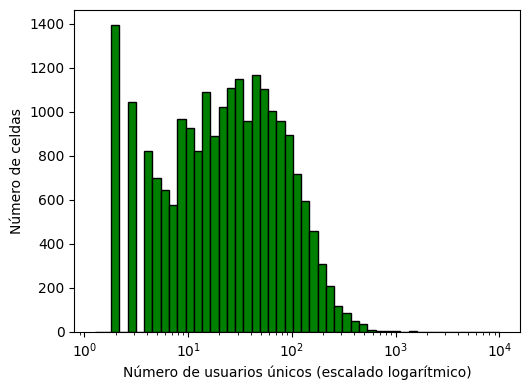
\includegraphics[width=\textwidth]{Graphics/unique_user_per_cell_histogram.png}
    \caption{Histograma del número de usuarios únicos por celdas.}
    \label{fig:unique_user_per_cell_histogram}
\end{minipage}%
\end{figure}

La figura \ref{fig:unique_user_per_day_plot} muestra la dinámica temporal del número usuarios únicos por día desde el día 0 hasta el 59. Los patrones muestran regularidad temporal, con patrones claros de días laborables y fines de semana. Hay una anomalía en el día 27, por tanto fueron excluidos del análisis los registros de ese día. La figura \ref{fig:ping_per_timeslot_plot} muestra la dinámica temporal del número de registros por intervalo de tiempo desde el intervalo 0 hasta el 47, agregados a lo largo de todos los días. Los patrones muestran regularidad temporal, con picos claros en la mañana y durante el día.

\begin{figure}[!htb]
\centering
\begin{minipage}{0.45\textwidth}
    \centering
    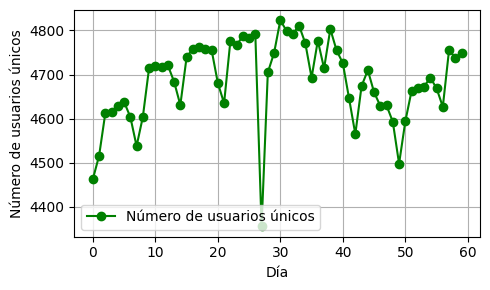
\includegraphics[width=\textwidth]{Graphics/unique_user_per_day_plot.png}
    \caption{Dinámica temporal del número de usuarios únicos por día.}
    \label{fig:unique_user_per_day_plot}
\end{minipage}%
\hfill
\begin{minipage}{0.45\textwidth}
    \centering
    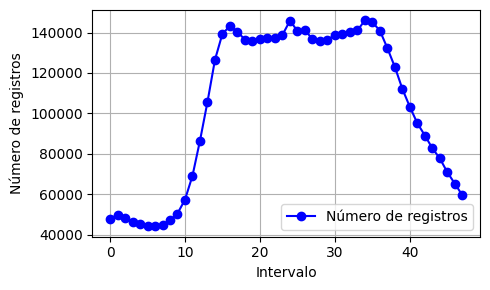
\includegraphics[width=\textwidth]{Graphics/ping_per_timeslot_plot.png}
    \caption{Dinámica temporal del número de registros por intervalo, agregados a lo largo de todos los días.}
    \label{fig:ping_per_timeslot_plot}
\end{minipage}%
\end{figure}

La figura \ref{fig:unique_user_per_cell_2_dimensional_histogram} (izquierda) muestra un histograma bidimensional en escala logarítmica del número de usuarios únicos por celda observados a lo largo de los 60 días de estudio. Los patrones muestran claramente áreas urbanas y rurales. Finalmente, se realizó una reducción de resolución al mapa de trayectorias discretizadas de 200 × 200 a 20 × 20, como se puede ver en la figura \ref{fig:unique_user_per_cell_2_dimensional_histogram} (derecha), lo cual disminuye significativamente el costo computacional al disminuir las celdas de 40,000 a 400, optimizando recursos y tiempos de ejecución, mientras preserva los patrones globales de densidad de usuarios y registros al sumar los valores agrupados, manteniendo la representatividad del comportamiento general.

\begin{figure}[!htb] \centering 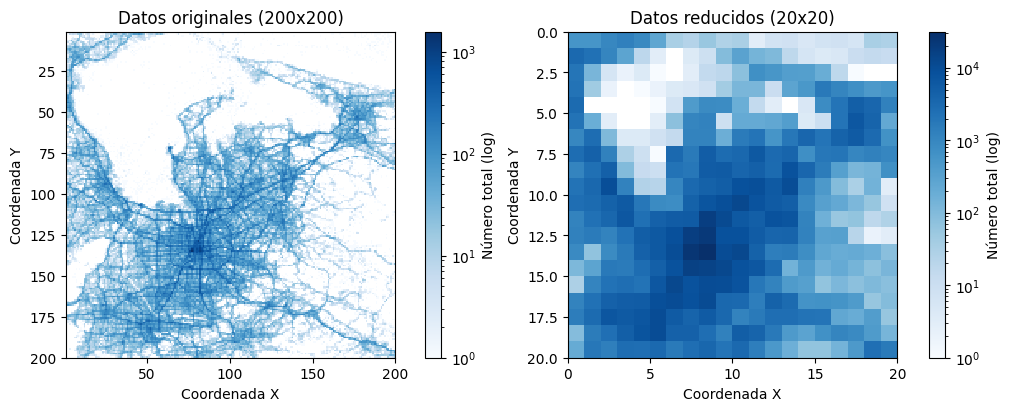
\includegraphics[width=1\textwidth]{Graphics/unique_user_per_cell_2_dimensional_histogram.png} \caption{Histograma bidimensional del número de usuarios únicos por celda. Datos originales a la izquierda, reducidos a la derecha.} \label{fig:unique_user_per_cell_2_dimensional_histogram} 
\end{figure}

\subsection{Experimentos}

El objetivo principal del experimento es validar la efectividad de la arquitectura propuesta por \textbf{TrajBert} para el completamiento de trayectorias en un conjunto de datos real, así como examinar el rendimiento de la función de pérdida y del refinamiento espaciotemporal propuesto en \cite{si2023trajbert}, evaluando la robustez del método con diversos grados de escasez de datos.

Para evaluar la superioridad de \textbf{TrajBERT}, se comparó con tres modelos base. El primer par de modelos son heurísticos, basados en conocimiento previo sobre patrones de movilidad humana, mientras que \textbf{BERT} es un modelo típico para procesar datos secuenciales. La descripción de los modelos base es la siguiente:

\begin{itemize}
    \item \textbf{Histórico:} Utiliza las ubicaciones más populares de cada usuario en cada intervalo de tiempo histórico para realizar la recuperación.
    \item \textbf{Top:} Utiliza las ubicaciones más populares de cada usuario a lo largo de todas las trayectorias históricas para realizar la recuperación.
    \item \textbf{BERT:} Desactivamos el refinamiento espaciotemporal y la función STAL de \textbf{TrajBERT}, manteniendo únicamente el codificador Transformer y el modelo de lenguaje enmascarado (MLM) para recuperar las ubicaciones omitidas. \ref{def:e_sampling}
\end{itemize}

El conjunto de trayectorias fue particionado en conjuntos de entrenamiento, validación y prueba en un 70\%, 15\% y 15\% respectivamente. En cada trayectoria de entrenamiento, validación y prueba se enmascaró el 15\% de las ubicaciones efectivas. Los valores $\epsilon, m$ definidos en \ref{def:e_sampling} se pusieron en 30 minutos y 48 intervalos respectivamente, haciendo las 24 horas del día. Los hiperparámetros \(\gamma\), \(\mu\) y \(\eta\) de la ecuación \ref{eq:w_loc_cases} se establecieron en 98, 1000 y $exp(1)$. \(\beta_1\) y \(\beta_2\) de la ecuación \ref{eq:stal}. Adicionalmente, la tasa de aprendizaje se estableció en $10^{-4}$, el tamaño del lote en 256, la cantidad de cabezas de atención en 8, la cantidad de capas en 6, el tamaño del \textit{embedding} en 512 y se usó el optimizador Adam. El entrenamiento se llevó a cabo en una laptop Acer Nitro ANV15-51 con Windows 11 Home 64-bit, procesador Intel Core i7-13620H (16 CPUs, ~2.4GHz) y 16GB de RAM.

Para evaluar el rendimiento de recuperación, se emplean las métricas \textbf{recall@k}
% , \textbf{mean Average Precision (mAP)} 
y la \textbf{media de la distancia de Manhattan}:

\begin{itemize}
    \item \textbf{Recall@k:} Si el ID de localización verdadero aparece dentro de los primeros $k$ resultados predichos, el valor de recall@k es 1, de lo contrario, es 0. El recall@k final es el cociente entre las predicciones correctas y el total de localizaciones enmascaradas. Se reportan valores de recall@k con $k=1$ y $k=3$.
    % \item \textbf{mAP:} Es una métrica global utilizada para evaluar la calidad del ranking completo.
    \item \textbf{Distancia de Manhattan:} Es una métrica utilizada para evaluar la proximidad entre las ubicaciones predichas y las ubicaciones reales en términos de su distancia geográfica. Calcula el promedio de las suma de las diferencias absolutas entre las coordenadas de dos puntos (latitud y longitud). Podemos usar esta métrica debido a la forma matricial que tienen nuestros datos \ref{fig:humob_matrix_mobility}.
\end{itemize}

Valores más altos de recall@k y mAP y más bajos en la media de la distancia de manhattan indican un mejor rendimiento del modelo. Además, \cite{si2023trajbert} introduce una métrica llamada \textbf{fuzzy accuracy (fuzzy-acc)} para evaluar la capacidad del modelo de recuperar rutas de movimiento reales. La \textit{fuzzy-acc} considera \textit{IDs de ubicaciones} geográficamente cercanas como válidas para evitar penalizaciones innecesarias. La \textit{fuzzy-acc} se define como:

\begin{equation}
    \text{fuzzy-acc} = 
    \begin{cases} 
    1, & \text{si } \text{predicción} \in C_{i,j} \\
    0, & \text{en otro caso}
    \end{cases}
\end{equation}
 
\noindent
donde $C_{i,j}$ es el conjunto de \textit{IDs de ubicación} similares al valor verdadero $t_{i,j}$, definido como:

\begin{equation}
    C_{i,j} = \bigcup \{k \,|\, H[t_{i,j}][k] > \gamma\}
\end{equation}

\noindent
aquí, $H$ es la matriz de co-ocurrencia \ref{eq:co_ocurrence_matrix} de todos los \textit{IDs de ubicación} y $\gamma$ es el umbral de co-ocurrencia usado en la ecuación \ref{eq:w_loc_cases}. 

La tabla \ref{tab:model_comparison} muestra el rendimiento de los modelos base y \textbf{TrajBERT}, con un 15\% de ubicaciones efectivas enmascaradas. El desempeño de los métodos \textbf{Histórico} y \textbf{Top} es bastante limitado debido a su incapacidad de aprender patrones complejos de movilidad, sin embargo la cantidad de datos permitió lograr una precisión cercana al 40\% en ambos casos. Aunque \textbf{BERT} no fue diseñado específicamente para el completamiento de trayectorias, el experimento evidencia que el uso de la red \textit{feed-forward} y la conexión residual en el \textit{encoder} puede generar resultados satisfactorios.

\textbf{TrajBERT} obtiene mejores resultados que el resto de los modelos base con un margen significativo. Comparado con \textbf{BERT}, \textbf{TrajBERT} mejora el \textit{encoder} Transformer mediante un refinamiento espaciotemporal y una función de pérdida consciente del espacio y el tiempo. Por un lado, el refinamiento espaciotemporal refuerza la importancia de los \textit{ID de ubicación} visitados recientemente y por visitar, y por otro lado, la función de pérdida incorpora información espacial global, ya que las trayectorias están restringidas por la topología de la ciudad. Los últimos tres registros de la tabla \ref{tab:model_comparison} presentan resultados que validan el uso del refinamiento espaciotemporal y la función STAL.

\begin{table}[ht]
\centering
\begin{tabular}{|l|c|c|c|c|}
\hline
\textbf{Modelo} & \textbf{Precisión} & \textbf{Fuzzy} & \textbf{Top 3}         &  \textbf{Manhattan}   \\ \hline
Top                  & 0.3924         & -                    & -               &       -               \\ \hline
Histórico            & 0.4162         & -                    & -               &       -               \\ \hline
Bert                 & 0.5415         & 0.7927             & 0.5580            &     2.1248            \\ \hline
TrajBert sin temp    & 0.5784         & 0.8276             & 0.6887            &     1.9426            \\ \hline
TrajBert sin STAL    & 0.6021         & 0.9128             & 0.7882            &     1.7268            \\ \hline
TrajBert             & 0.6104         & 0.9141             & 0.7980            &     1.7044            \\ \hline
\end{tabular}
\captionof{table}{Comparación de resultados de los modelos}
\label{tab:model_comparison}
\end{table}

% & \textbf{MAP}
%      & -      
%      & -      
%  & 0.4651     
%  & 0.6432     
%  & 0.7091     
%  & 0.7169  

Se evaluó la robustez de \textbf{TrajBERT} frente a diferentes escenarios de escasez de datos, configurando la tasa de ocultamiento del conjunto de prueba entre 10\% y 90\%. La tasa de ocultamiento se define como el número de ubicaciones efectivas eliminadas intencionalmente para disminuir la información del contexto y evaluar la capacidad del modelo de recuperar las enmascaradas. La tasa de pérdida se calcula con la siguiente fórmula:

\begin{equation}
\text{Tasa de pérdida} = \frac{n_{\text{mask}} + n_{\text{pad}} + n_{\text{hid}}}{m}
\end{equation}

\noindent
donde $n_{\text{mask}}$ es el número de ubicaciones enmascaradas, $n_{\text{hid}}$ es el número de ubicaciones ocultadass, $n_{\text{pad}}$ es el número de ubicaciones desconocidas y marcadas como \textit{padding}, y $m$ es el total de intervalos de tiempo.

El modelo \textbf{TrajBERT} demostró una notable capacidad de recuperación, manteniendo un rendimiento destacado incluso con tasas de pérdida superiores al 80\%. En estos escenarios, logró predecir correctamente más del 50\% de las ubicaciones enmascaradas, mostrando su eficacia en condiciones de datos altamente escasos. Se puede apreciar el comportamiento de las métricas de evaluación del modelo en la figura \ref{fig:humob_percent_variability_analisys}.

\begin{figure}[!htb] 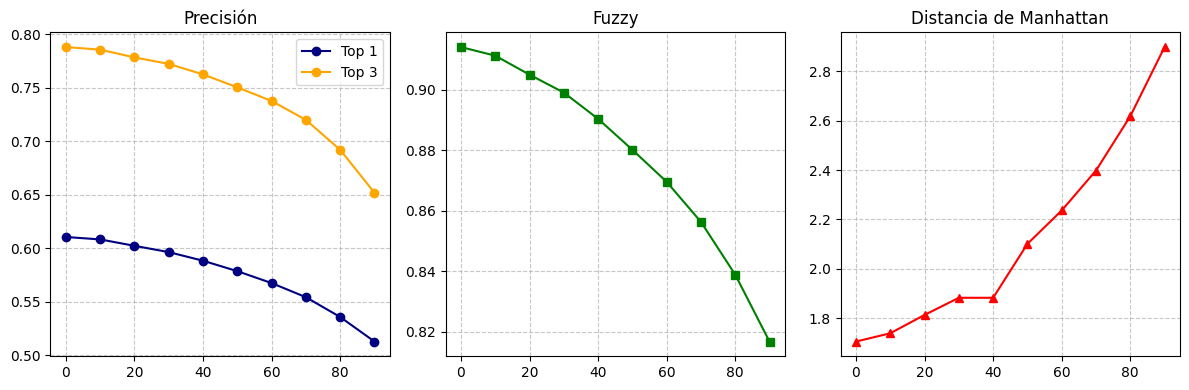
\includegraphics[width=1\textwidth]{Graphics/humob_percent_variability_analisys.png} \caption{Relación entre el porcentaje de datos ocultos y el desempeño del modelo. Cada gráfico muestra cómo varía una métrica específica al incrementar el nivel de enmascaramiento en las trayectorias.} \label{fig:humob_percent_variability_analisys} 
\end{figure}

% \subsection{Conclusiones}